 % -*- root: ../main.tex -*-
\documentclass[../main.tex]{subfiles}
\begin{document}

\chapter{Publications}\label{chap:publications}

\clearpage
\newpage

% ================================================

\section{Mécanismes d'action des récepteurs aux hormones thyroïdiennes durant le développement : Lessons retenues des études sur les amphibiens}\label{sec:bba-review}

\begin{abstract}
Les \glspl{tr} jouent un rôle critique durant le développement des vertébrés.
Cependant, leur mécanismes d'action \textit{in vivo} reste peu exploré.
Cette revue catalogue certains des résultats obtenus dans le contexte de la métamorphose des amphibies sur les fonctions développementales des \glspl{ht} et des \glspl{tr} et leur mécanismes associés.
\par
Un modèle de double fonction de \gls{tr} pour le développement des Anoures a été proposé il y a près d'une décade.
Selon ce modèle, \gls{tr} non lié à son ligand recrute des complexes co-répresseurs – contenant des désacétylases d'histones – au niveau de gènes cibles des \glspl{ht} durant la pré-métamorphose pour réprimer l'expression de ces gènes et empêcher la métamorphose prématurée.
Par la suite, quand les \glspl{ht} sont disponibles, \gls{tr} lié au ligand recrute des complexes co-activateurs – contenant des modificateurs d'histones et des remodeleurs de la chromatine – pour cette fois activer l'expression de ces même gènes et induire les changements associés à la métamorphose.
Ces complexes peuvent altérer la structure de la chromatine par déplacement ou éviction des nucléosomes et la modification d'histones, contribuant au recrutement de la machine transcriptionnelle et à l'activation de gènes.
\par
Les mécanismes moléculaires impliqués dans ce modèle sont très probablement transposables à des modèles mammaliens.
\end{abstract}

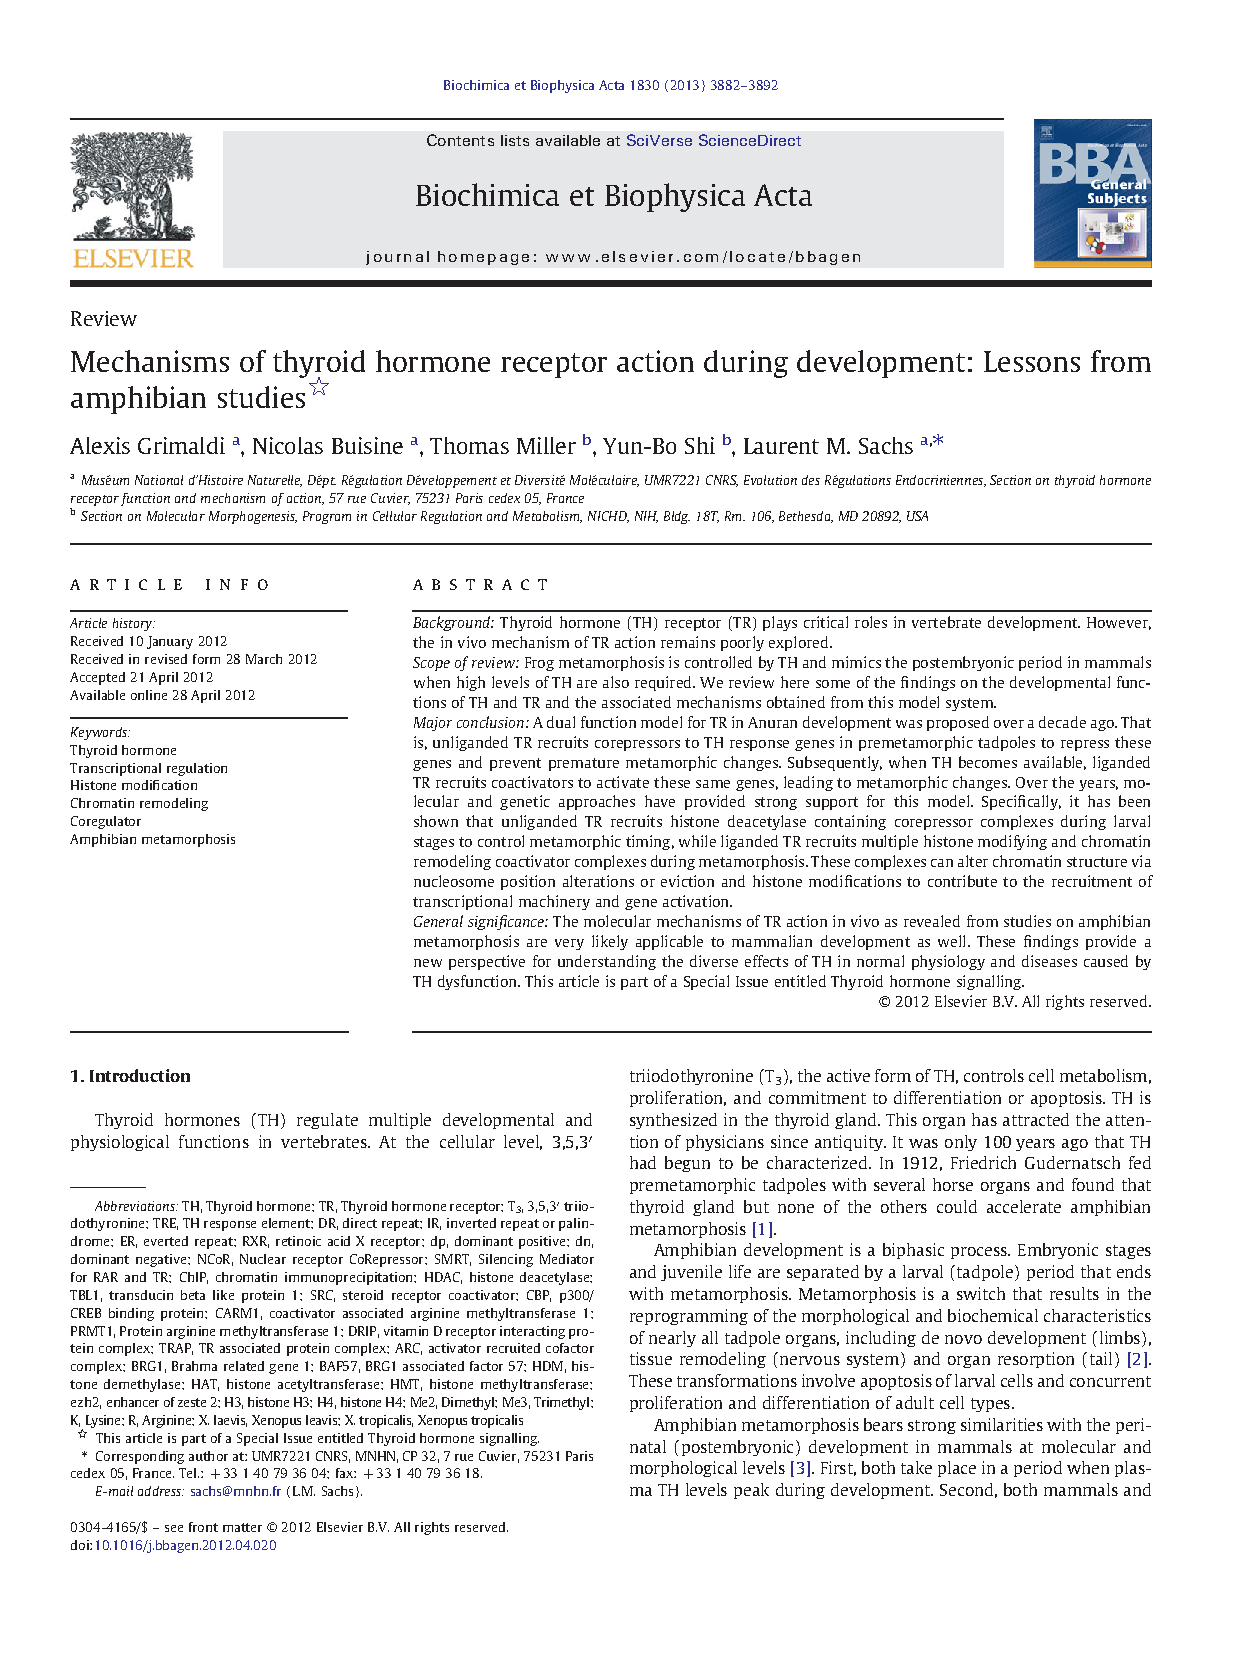
\includepdf[pages={-}]{Publications/bba-review.pdf}

% ====================================================

\clearpage
\newpage

% ====================================================

\section{Les technologies de séquençage à haut débit vont métamorphoser l'analyse de la fonction des récepteurs aux hormones thyroïdiennes pendant le développement de l'amphibien}\label{sec:ctdb-review}

\begin{abstract}
La métamorphose des amphibiens est marquée par des changement spéctaculaires induits par les \glspl{ht}, incluant de la morphogenèse, le remodelage de tissus et la résorption de tissus par mort cellulaire programmée.
\par
Les \gls{ht} agissent via leur récépteurs, les \glspl{tr}.
En abscence d'hormone, ceux-ci recrutent des complexes co-répresseurs au niveau des gènes cibles.
Ces complexes co-répresseurs sont échangés pour des complexes co-activateurs en présence d'hormone.
Afin de pleinement comprendre la diversité des effets de la \glspl{t3} durant la métamorphose, l'analyse du transcriptome et des mécanismes d'action de \gls{tr} à l'échelle du génome est nécessaire.
\par
Les nouvelles technologies de séquençage ont profondément changé la façon dont de nouvelle questions fondamentales sont abordées, et font maintenant partie des standards utilisés en génomique et en génomique fonctionnelle.
\par
Cette revue se concentre sue les applications des nouvelles technologies de séquençage pour l'analyse et l'exploration de la métamorphose des amphibiens.
\end{abstract}

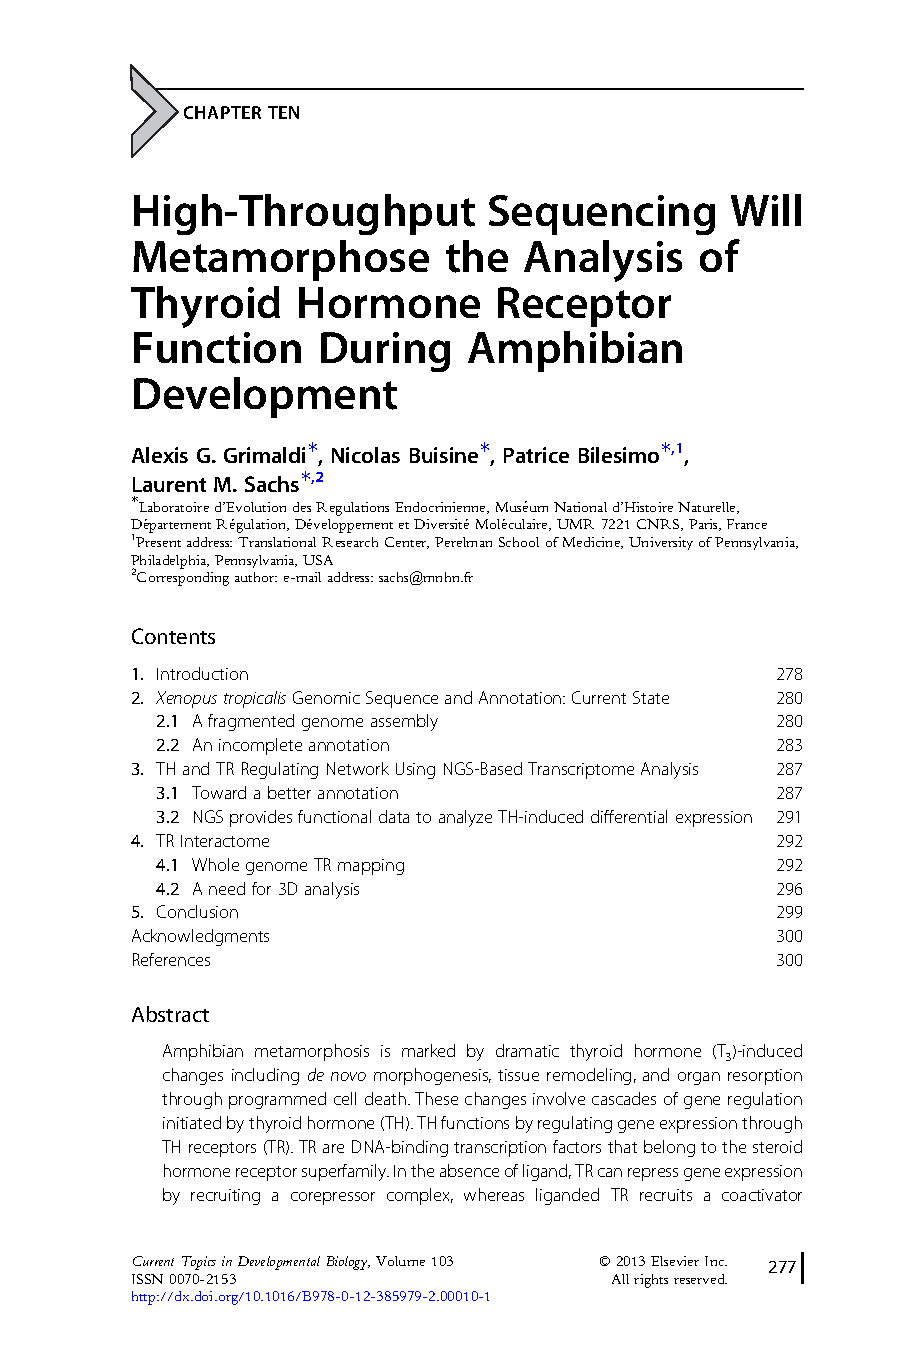
\includepdf[pages={-},nup=1x2,landscape=true]{Publications/ctdb-review.pdf}
% 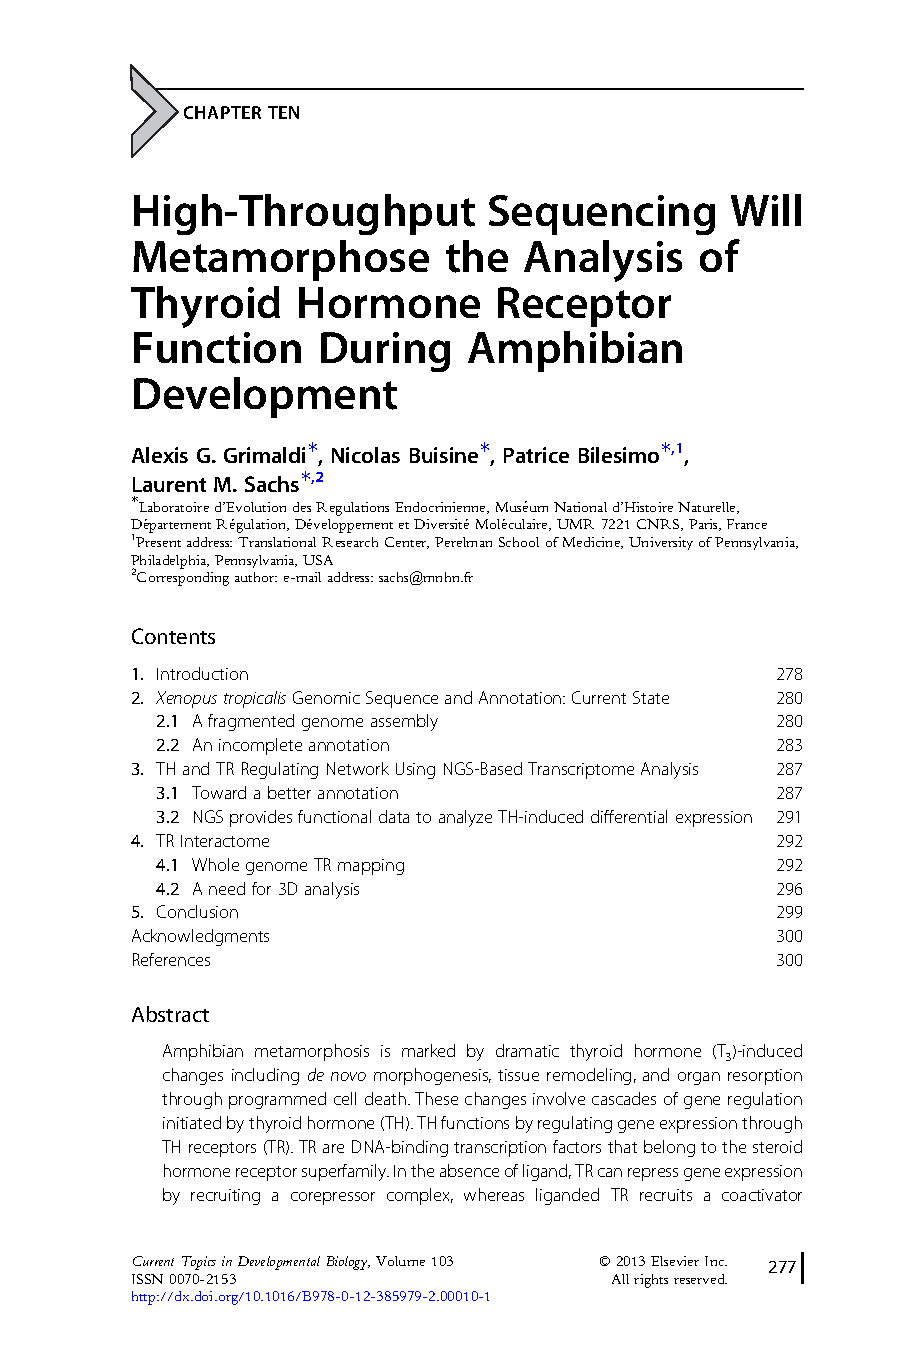
\includepdf[pages={-}]{Publications/ctdb-review.pdf}

\clearpage
\newpage

\section{Re-assembly and re-annotation of the Xenopus tropicalis genome for in vivo ChIA-PET analysis}\label{sec:buisine2014}

\begin{abstract}

Abstract

\end{abstract}

% 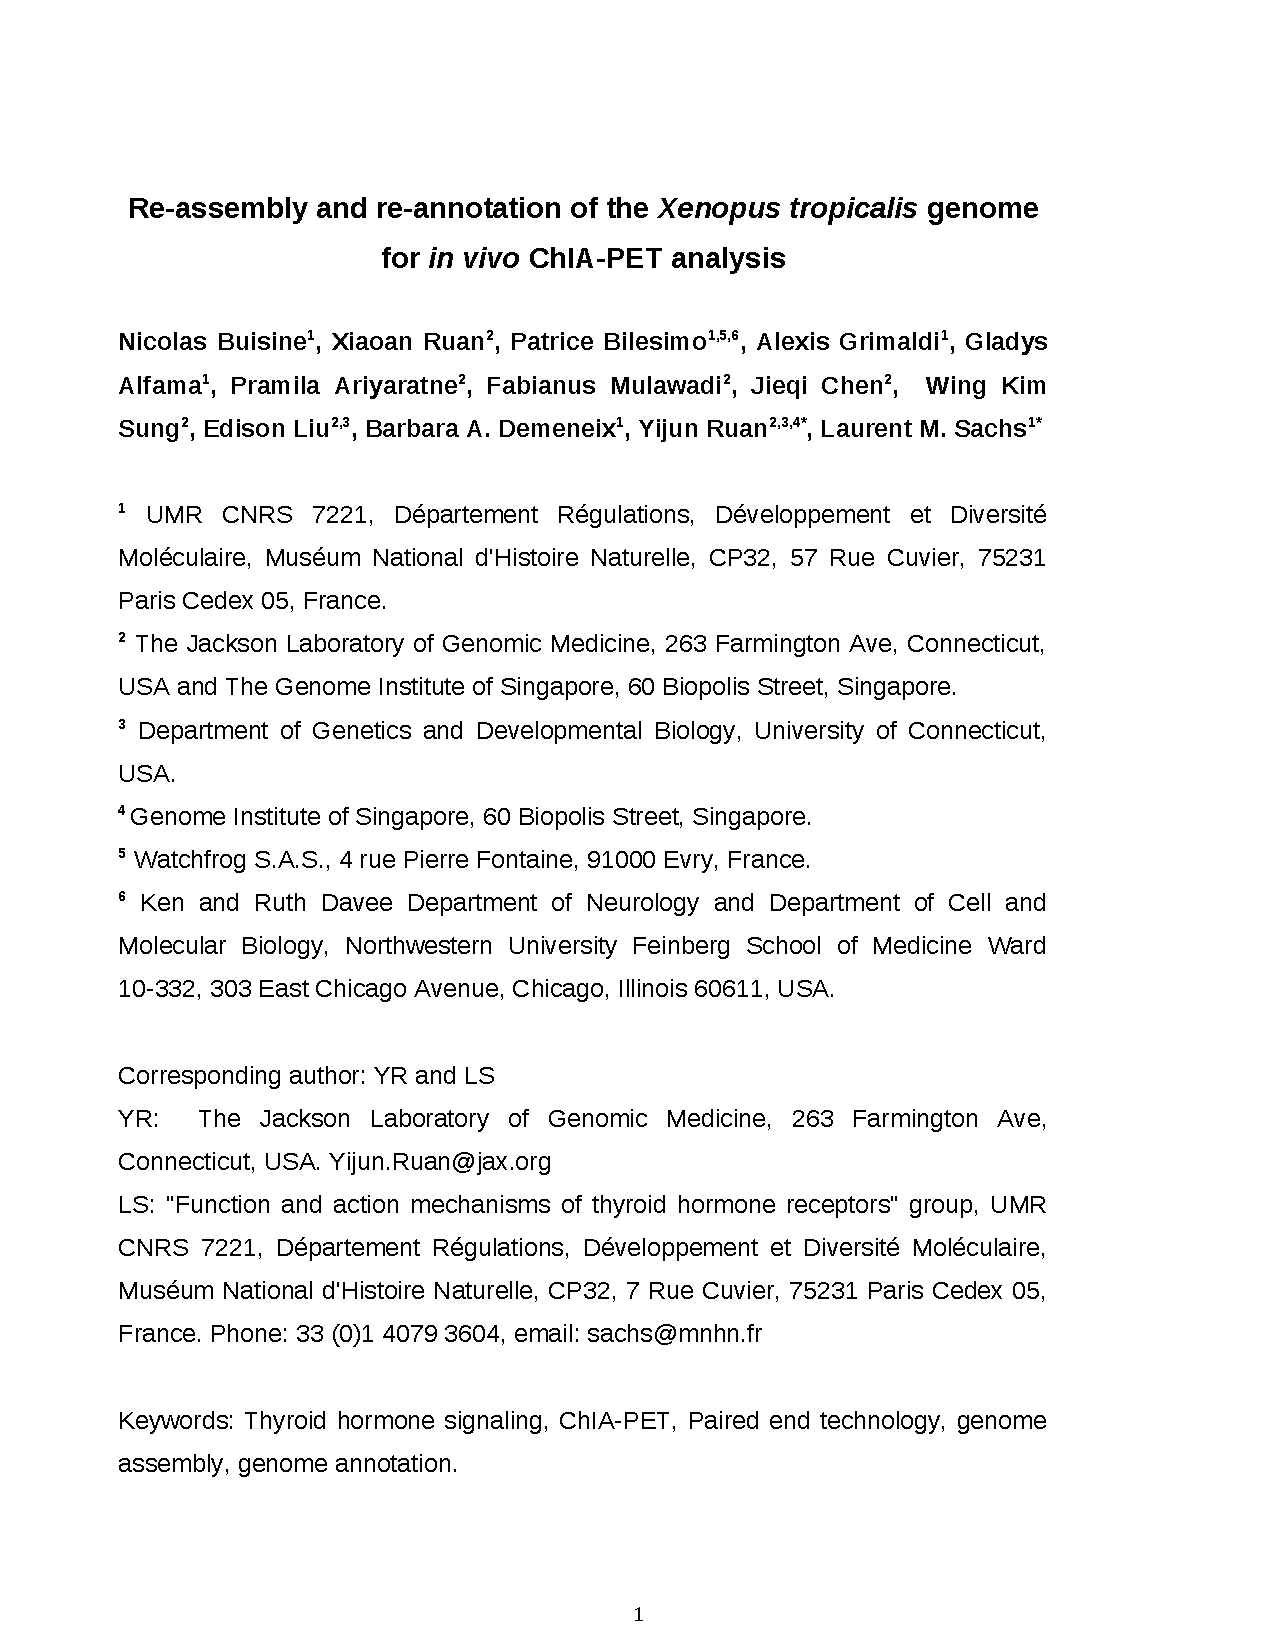
\includepdf[pages={-}]{Publications/buisine2014.pdf}
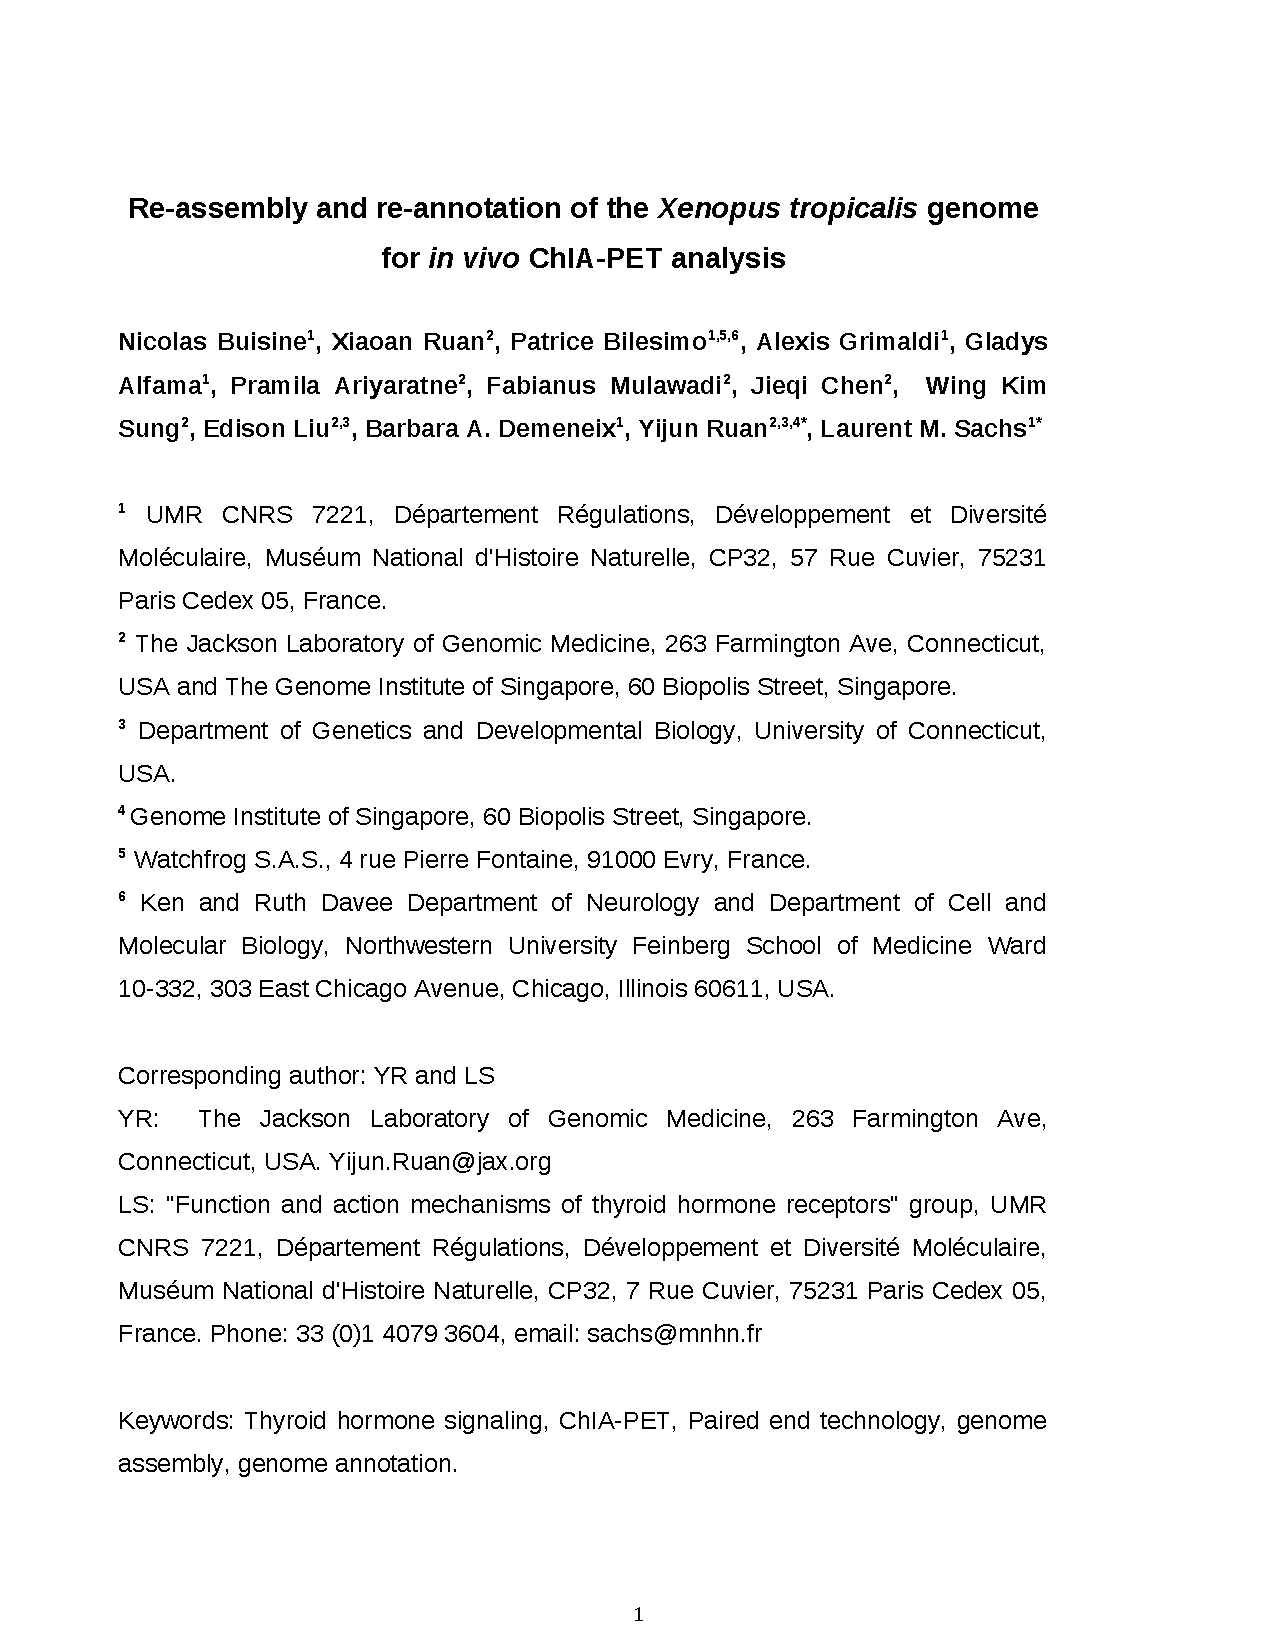
\includepdf[pages={-},nup=1x2,landscape=true]{Publications/buisine2014.pdf}
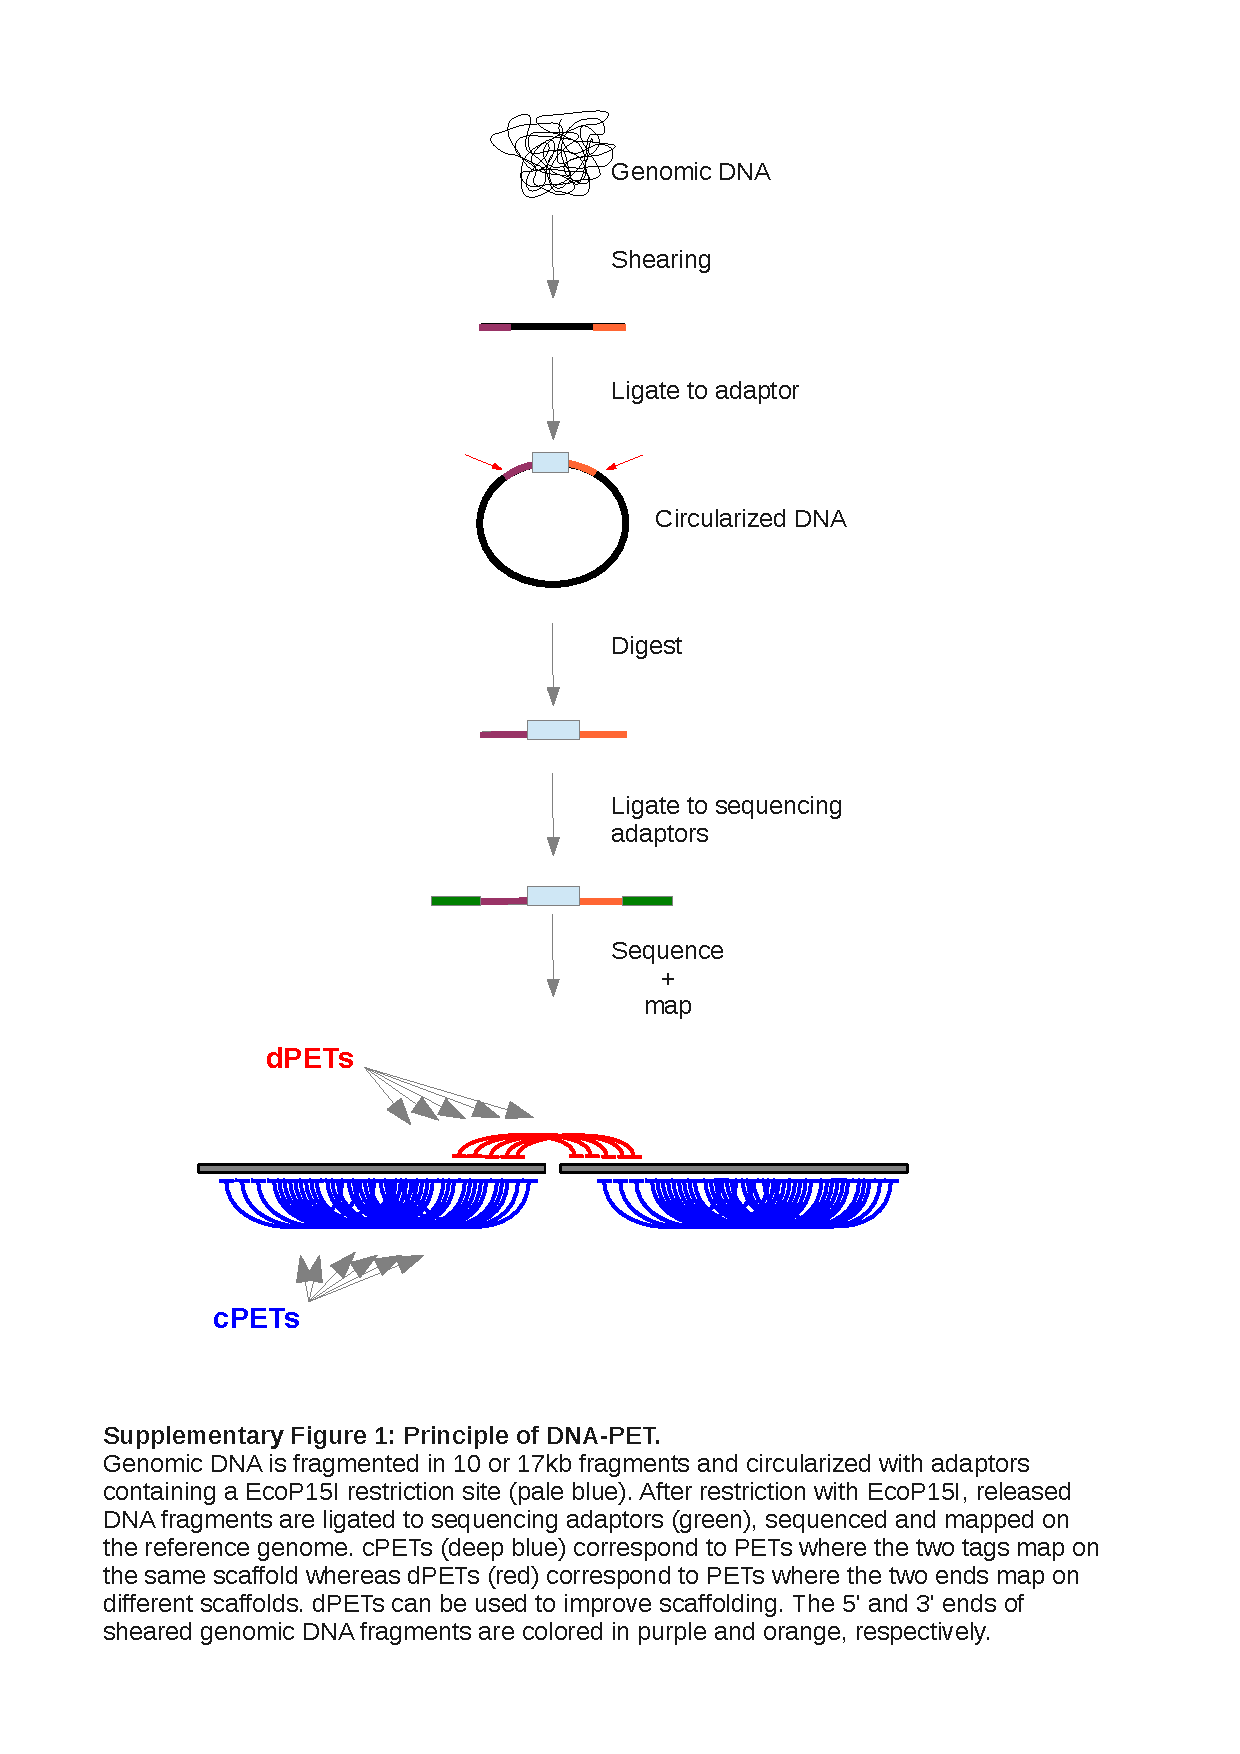
\includepdf[pages={-},nup=1x2,landscape=true]{Publications/buisine2014-sup.pdf}

\end{document}